

\tikzset{every picture/.style={line width=0.75pt}} %set default line width to 0.75pt        

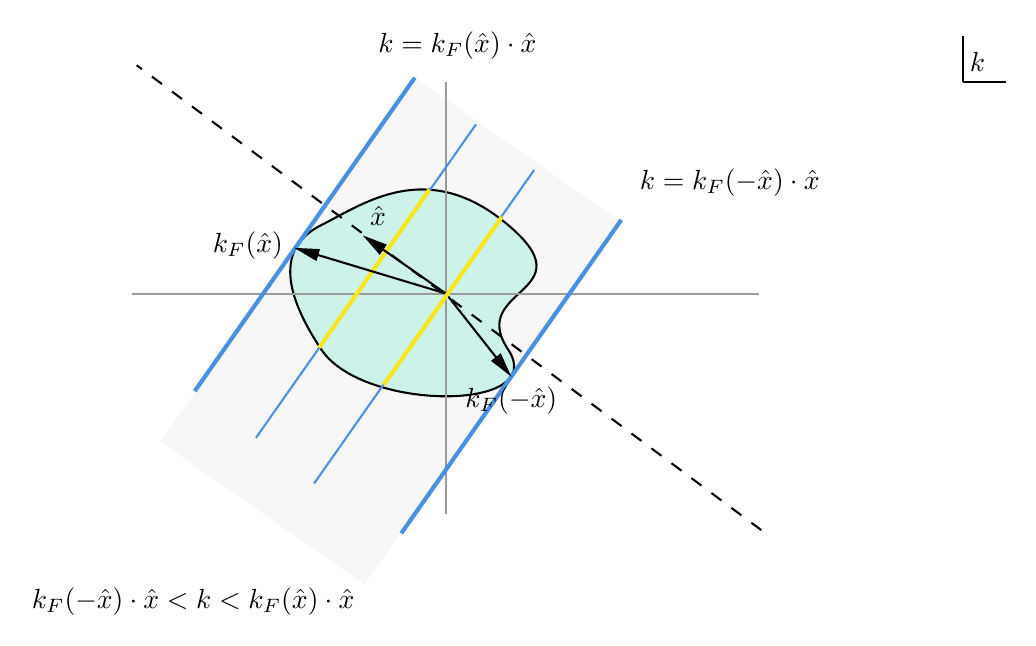
\begin{tikzpicture}[x=0.75pt,y=0.75pt,yscale=-1,xscale=1]
%uncomment if require: \path (0,369); %set diagram left start at 0, and has height of 369

%Shape: Rectangle [id:dp7890850960485711] 
\draw  [draw opacity=0][fill={rgb, 255:red, 155; green, 155; blue, 155 }  ,fill opacity=0.08 ] (150.46,216.46) -- (273,41) -- (371.39,109.71) -- (248.85,285.17) -- cycle ;
%Shape: Polygon Curved [id:ds16933255681931936] 
\draw  [fill={rgb, 255:red, 80; green, 227; blue, 194 }  ,fill opacity=0.26 ] (228,112) .. controls (248,102) and (279,79) .. (318,112) .. controls (357,145) and (298,142) .. (318,172) .. controls (338,202) and (248,202) .. (228,172) .. controls (208,142) and (208,122) .. (228,112) -- cycle ;
%Straight Lines [id:da8172830438322201] 
\draw [color={rgb, 255:red, 155; green, 155; blue, 155 }  ,draw opacity=1 ]   (137,145) -- (439,145) ;
%Straight Lines [id:da8464582519121175] 
\draw [color={rgb, 255:red, 155; green, 155; blue, 155 }  ,draw opacity=1 ]   (288,251.25) -- (288,43) ;
%Straight Lines [id:da6926385458902968] 
\draw  [dash pattern={on 4.5pt off 4.5pt}]  (440,259) -- (139,35) ;
%Straight Lines [id:da01759015854493362] 
\draw [color={rgb, 255:red, 74; green, 144; blue, 226 }  ,draw opacity=1 ][line width=1.5]    (273,41) -- (167,192) ;
%Straight Lines [id:da14995718249679646] 
\draw [color={rgb, 255:red, 74; green, 144; blue, 226 }  ,draw opacity=1 ]   (302.5,63.5) -- (196.5,214.5) ;
%Straight Lines [id:da4192220598532561] 
\draw [color={rgb, 255:red, 74; green, 144; blue, 226 }  ,draw opacity=1 ]   (330.5,85.5) -- (224.5,236.5) ;
%Straight Lines [id:da6663112276637151] 
\draw [color={rgb, 255:red, 74; green, 144; blue, 226 }  ,draw opacity=1 ][line width=1.5]    (372.5,109.5) -- (266.5,260.5) ;
%Straight Lines [id:da48007887551929507] 
\draw    (537,43) -- (558,43) ;
%Straight Lines [id:da8390776098943569] 
\draw    (537,43) -- (537,21) ;
%Straight Lines [id:da41530809059346585] 
\draw    (288,145) -- (318.26,183.43) ;
\draw [shift={(319.5,185)}, rotate = 231.78] [fill={rgb, 255:red, 0; green, 0; blue, 0 }  ][line width=0.08]  [draw opacity=0] (12,-3) -- (0,0) -- (12,3) -- cycle    ;
%Straight Lines [id:da7596590644475403] 
\draw [color={rgb, 255:red, 248; green, 231; blue, 28 }  ,draw opacity=1 ][line width=1.5]    (227,171) -- (280,95) ;
%Straight Lines [id:da33448048650418194] 
\draw    (288,145) -- (249.64,118.15) ;
\draw [shift={(248,117)}, rotate = 34.99] [fill={rgb, 255:red, 0; green, 0; blue, 0 }  ][line width=0.08]  [draw opacity=0] (12,-3) -- (0,0) -- (12,3) -- cycle    ;
%Straight Lines [id:da08297341295296312] 
\draw    (288,145) -- (216.91,123.58) ;
\draw [shift={(215,123)}, rotate = 16.77] [fill={rgb, 255:red, 0; green, 0; blue, 0 }  ][line width=0.08]  [draw opacity=0] (12,-3) -- (0,0) -- (12,3) -- cycle    ;
%Straight Lines [id:da2776423007341342] 
\draw [color={rgb, 255:red, 248; green, 231; blue, 28 }  ,draw opacity=1 ][line width=1.5]    (258,189) -- (315,108) ;

% Text Node
\draw (250,113.6) node [anchor=south west] [inner sep=0.75pt]    {$\hat{\boldsymbol{x}}$};
% Text Node
\draw (211,122) node [anchor=east] [inner sep=0.75pt]    {$\boldsymbol{k}_{\text{F}}(\hat{\boldsymbol{x}})$};
% Text Node
\draw (254,17.4) node [anchor=north west][inner sep=0.75pt]    {$k=\boldsymbol{k}_{\text{F}}(\hat{\boldsymbol{x}}) \cdot \hat{\boldsymbol{x}}$};
% Text Node
\draw (539,39.6) node [anchor=south west] [inner sep=0.75pt]    {$\boldsymbol{k}$};
% Text Node
\draw (380,83.4) node [anchor=north west][inner sep=0.75pt]    {$k=\boldsymbol{k}_{\text{F}}( -\hat{\boldsymbol{x}}) \cdot \hat{\boldsymbol{x}}$};
% Text Node
\draw (319.5,188.4) node [anchor=north] [inner sep=0.75pt]    {$\boldsymbol{k}_{\text{F}}( -\hat{\boldsymbol{x}})$};
% Text Node
\draw (87,285.4) node [anchor=north west][inner sep=0.75pt]    {$\boldsymbol{k}_{\text{F}}( -\hat{\boldsymbol{x}}) \cdot \hat{\boldsymbol{x}} < k< \boldsymbol{k}_{\text{F}}(\hat{\boldsymbol{x}}) \cdot \hat{\boldsymbol{x}}$};


\end{tikzpicture}
